\chapter{Study II: Time-to-Event Prediction of All-Cause Mortality}
\label{chap:study2-outline}

\newcommand{\graceii}{\acsfont{GRACE 2.0}}

In this chapter, I provide a summary of the work from \studyii{}.
I describe the background and rationale,
outline essential methodological details,
and discuss the main research findings.

The manuscript, titled \enquote{%
Development and validation of a neural network-based survival model 
for mortality in ischemic heart disease}, 
is currently under review (2nd round).
An earlier version of the manuscript
has been deposited on the medRxiv preprint server. 
~\autocite{holmDevelopment2023}
The revised full-length manuscript is included in 
\cref{chap:study2-paper}.

\section{Background and Objectives}

For patients with \ac{IHD}, 
the use of risk stratification algorithms, 
which assess the presence or absence of prognostic
risk factors and disease indicators, 
can be crucial in tailoring patient-specific treatment approaches. 
\autocite{knuuti20192020}
\autocite{collet20202021}
\autocite{stegESC2012}
Notably, the revised \acsu{GRACE} risk score (\acsfont{GRACE 2.0}),
~\autocite{foxShould2014}
which has been widely adopted in the clinical setting and 
received a class IIa recommendation for assessing and managing patients
with \ac{NSTEMI} in recent \acsu{ESC} guidelines,
~\autocite{collet20202021}
serves as a prime example of such an algorithm.

Presently,
risk stratification algorithms for secondary prevention in \ac{IHD},
including \acsfont{GRACE 2.0}, 
are limited to a narrow range of established risk factors and are constructed
using traditional statistical methods like the Cox proportional hazards model
or logistic regression. 
These conventional models, while useful, 
have strong assumptions, lack flexibility, are imprecise, and are not well-suited
for integration of large and heterogenous arrays of predictors---%
at least not without extensive feature engineering and selection.

In this study, we hypothesised that prognostication models in \ac{IHD}
would benefit from the inclusion of a much wider array of features,
which is already available from \ac{EHR} systems in clinical use.
To enable the inclusion of such features, and also allow the modelling
of time-to-event outcomes with potential censoring, we set out 
use a neural network-based survival model. Specifically, the 
discrete time framework proposed by \textcite{gensheimerScalable2019}, 
which I have described in detail in \cref{chap:survival-analysis}.

Since this framework does not allow inclusion of competing risks,
we limited the scope of the study to only consider prediction
of all-cause mortality.

\section{Study Design}

For model development, we defined a retrospetive cohort from the \ac{LPR}
and \ac{EDHR} which consisted of \num{39746} adult patients with \ac{IHD}.

All patients in the cohort had their first \ac{CAG} performed between
1st of January 2006 and 7th of July 2016, which were required to 
have led to a diagnosis of one-, two-, or three-vessel disease 
(\acsfont{1-3VD}) or \ac{DA}.

We defined the index date as the date of the inclusion \ac{CAG}, and 
included five years of follow-up from the \ac{CPR}, which was used
to define all-cause mortality.

The development cohort was randomly split into a training set 
and a hold-out test set consisting of 
\num{34746} and \num{5000} patients, respectively.

For external validation, a cohort of \num{8287} Icelandic adults 
with \ac{IHD} who had undergone \ac{CAG} were similarly defined,
as detailed in the methods section of the manuscript 
(see \cref{chap:study2-paper}).

\section{Methodology}

Using the discrete time logistic-hazard approach described in 
\cref{chap:survival-analysis}, we trained neural network models
to predict the probability of all-cause mortality within five years
after the index \ac{CAG}.
The model output are discrete time conditional hazards, 
and as such, can be used to construct a survival function that
gives the estimated probability at any timepoint within the
prediction horizon.

Models were trained using only the training set, and the hyperparameters
were tuned using the \ac{HPO} library Optuna in Python.
~\autocite{akibaOptuna2019}
For the \ac{HPO}, we used 5-fold cross-validation to obtain a bias-corrected
estimate of the model performance.

Different intermediate models were trained using various combinations
of the included features listed in \cref{tab:pmhnet-1-features},
to explore their respective impact on model performance.
For the complete model, which we refer to as \pmhnet{1}, we included
all available features.

\begin{table}[htbp]% →
    \newcommand{\catbox}[1]{%
        \tikz [anchor=base, baseline=1pt] 
            \draw[fill=#1, rounded corners=1pt] (0,0) rectangle (2.6mm, 2.6mm);
    }
\small
\begin{tabularx}{\linewidth}{clX}\toprule
  & {Category} & Features \\\midrule
  \catbox{cln1} & ClinicalOne  & 
    age, pulse, systolic blood pressure, 
    cardiac arrest~(yes/no), abnormal cardiac enzymes~(yes/no),
    killip class, serum creatinine, \acsfont{ST}-segment deviation~(yes/no)
    \\
  \catbox{cln2} & ClinicalTwo  & 
    abnormal \acs{ECG}~(yes/no), \acs{CCS}, 
    diastolic blood pressure,
    coronary artery dominance, familial \ac{IHD}~(yes/no), height,
    weight, \acsfont{ICD}-device or pacemaker~(yes/no), ischemia test, 
    \acs{LVEF}, \acs{NYHA} class, sex~(male/female), smoking status, 
    coronary pathology (\acsfont{1-3VD} or \acs{DA})
  \\
  \catbox{diag} & Diagnoses    & 
  \num{322} different level-3 \acs{ICD-10} diagnosis codes 
  \\
  \catbox{proc} & Procedures   & 
  \num{154} \acs{NOMESCO} procedure codes corresponding to 
  different examinations and surgical procedures
  \\
  \catbox{bioc} & Biochemical  & 
  \num{85} different lab tests with results categorized as below, within, or
  above the reference range
  \\ \bottomrule
\end{tabularx}
\caption[Overview of \pmhnet{1} features]{%
    Overview of \pmhnet{1} input features.  The different features were 
    grouped into five different categories according to their respective 
    characteristics.
    The \enquote{clinical} features were separated into two different
    subgroups, where \enquote{ClinicalOne} consist of the exact same features
    as those used in the \acsfont{GRACE 2.0} score.}
\label{tab:pmhnet-1-features}
\end{table}
% ←

We evaluated model performance by assessing both model discrimination and
calibration. Model discrimination was quantified by calculation of 
\ac{tdAUC}, which has the same interpretation as the commonly used \(c\)-index,
but is instead appropriate to use for the evaluation of \(t\)-year predicted
risk, as described in \textcite{blancheCindex2019}.
We assessed model calibration by constructing calibration curves,
comparing model predictions with estimated actual risks,
and by computing the Brier score.
For these model evaluation metrics, 
we use the implementations provided by the R-package \texttt{riskRegression}.
~\autocite{gerdsMedical2021}
All performance metrics were exclusively calculated using 
the internal or external test set.

Model performance was compared to that of the \graceii{} risk score.
~\autocite{foxShould2014}
The \graceii{} score was calculated by extracting the source code from the 
\graceii{} webtool and deploying a local R-based equivalent.
~\autocite{GRACE}
Since \graceii{} does not allow missing values, 
and all eight variables it uses was only available for \qty{51.4}{\percent} 
of our cohort, we imputed missing values 
using the \texttt{missForest} method prior to calculation.
~\autocite{stekhovenMissForest2012}
Additionally, since \graceii{} is not explicitly developed to provide
predictions at the index time used in our study, we also trained a 
neural network that was limited to consider only the \graceii{} features
(corresponding to the \enquote{ClinicalOne} features in 
\cref{tab:pmhnet-1-features}), which I will refer to as \graceii{} (re-fitted).
In this model, as well as in \pmhnet{1}, missing features were left 
missing as the neural network was designed to handle such.

Lastly, to provide model explanations and further investigate indvidual
features' impact on the model predictions, we performed \acsu{SHAP} 
analyses. \ac{SHAP} is a model-agnostic approach that can provide
measures of feature importance in otherwise \enquote{black-box} \ac{ML} 
models (see \cref{sub:what-is-shap}).


% figure: calibration curves→
\begin{marginfigure}
    \centering
    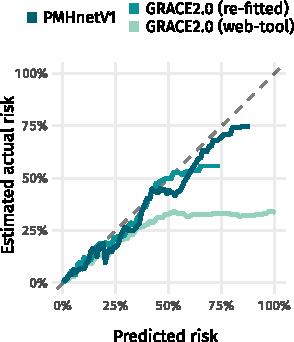
\includegraphics[trim=3mm 0 0 0, width=0.8\textwidth]{graphics/pmhnetv1-performance-curves.pdf}
    \caption[Calibration curves for \pmhnet{1} and \acs{GRACE} 2.0]{%
        Calibration curve for the \pmhnet{1} model and
        the \acs{GRACE} 2.0 reference models at a prediction
        horizon of three years.%
        %(\,\cbox{color1}{\phantom{a}}\,) {\pmhnet{1}},
        %(\,\cbox{color2}{\phantom{a}}\,) {\acs{GRACE} (re-fitted)}, and
        %(\,\cbox{color3}{\phantom{a}}\,) {\acs{GRACE} (web-tool)},
    }
    \label{fig:pmhv1-curves}
\end{marginfigure}% ←

\section{Main Findings}

From the model evaluation, we found the \pmhnet{1} model to provide excellent
model discrimination, outperforming both the standard \graceii{} score and
our neural network model using the \graceii{} features 
(\cref{tab:pmhv1-discrimination}).
We also found the model to be well calibrated as exemplified by 
\cref{fig:pmhv1-curves}, which shows the calibration curves for the 
3-year predictions. The \graceii{} score was miscalibrated, but our
re-fitted version had comparable calibration to the \pmhnet{1} model.

% table: auc scores→
\begin{table}[b]
\newcommand{\sici}[2]{(\num{#1}--\num{#2})}
\newcommand{\cii}{(\textlf{95\%CI})}
\newcommand{\gracw}{\acsfont{GRACE 2.0} (web tool)}
\newcommand{\gracn}{\acsfont{GRACE 2.0} (re-fitted)}
\newcolumntype{Y}{>{\centering\arraybackslash}X}
\addtolength{\tabcolsep}{-.55em}
\footnotesize
\begin{tabularx}{\linewidth}{Xcccccccc}\toprule
           & \multicolumn{2}{c}{6 months} & \multicolumn{2}{c}{1 year} & \multicolumn{2}{c}{3 years} & \multicolumn{2}{c}{5 years} \\
             \cmidrule(lr){2-3}             \cmidrule(lr){4-5}           \cmidrule(lr){6-7}            \cmidrule(lr){8-9}
           & \ac{tdAUC} & \cii{}          & \ac{tdAUC} & \cii{}        & \ac{tdAUC}    & \cii{}      & \ac{tdAUC} & \cii{}         \\\midrule
\pmhnet{1} & 0.88 & \sici{.86}{.90}       & 0.88 & \sici{.86}{.90}     & 0.84 & \sici{.82}{.86}      & 0.82 & \sici{.80}{.84}      \\
\gracw{}   & 0.77 & \sici{.74}{.80}       & 0.77 & \sici{.74}{.80}     & 0.73 & \sici{.71}{.75}      & --   & --                   \\
\gracn{}   & 0.79 & \sici{.76}{.83}       & 0.78 & \sici{.75}{.81}     & 0.76 & \sici{.74}{.78}      & --   & --                   \\\bottomrule
\end{tabularx}
\caption[\acs{tdAUC} of \pmhnet{1} and the \graceii{} Risk Score][-1.5em]{%
    \acsu{tdAUC} scores for \pmhnet{1}, \graceii{} (web tool), 
    and \graceii{} (re-fitted) at four different prediction horizons.
    The standard \graceii{} score does not predict 5-year survival and
    an \ac{tdAUC} was therefore not calculated at that prediction horizon.}
\label{tab:pmhv1-discrimination}
\end{table}% ←

To further assess the generalisability of the model, 
we performed external validation on an Icelandic cohort of \num{8287} patients.
Due to data availability, we used a slightly down-scaled version of the model 
that was limited to the \num{404} features that could be obtained from 
the Icelandic data. In the internal test set, the \ac{tdAUC} of this model
was 0.87 (\num{.85}--\num{0.90}) for the 6 month prediction,
0.87 (\num{.85}--\num{0.89}) for the 1 year prediction,
and 0.82 (\num{.80}--\num{0.85}) for the 3 year prediction.
On the Icelandic data, the \ac{tdAUC}
was 0.87 (\num{.84}--\num{0.90}) for the 6 month prediction,
0.84 (\num{.81}--\num{0.87}) for the 1 year prediction,
and 0.81 (\num{.79}--\num{0.85}) for the 3 year prediction.
We acknowledge that 
model performance can not directly be compared across cohorts,
but this qualitatively shows that 
model discrimination remained high in an external dataset.

To examine the effect of including different types of features,
we calculated \ac{tdAUC} of different intermediate models limited to
only consider certain combinations of feature modalities.
These results are presented in \cref{fig:category-overview} and shows 
that performance increased with increasing number of features,
however, with diminishing incremental gains.

% figure: intermediate models→
\begin{figure}[htb]
    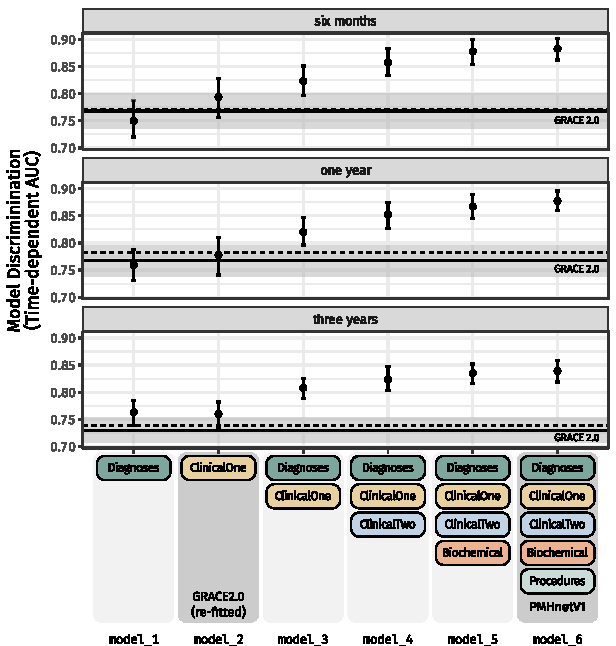
\includegraphics[trim=5mm 8mm 0 0]{graphics/pmhnet-v1-category-overview.pdf}
    \caption[Performance of intermediate \pmhnet{1} models]{%
        \acs{tdAUC} scores of different intermediate \pmhnet{1} models each
        limited to specific combinations of the designated feature categories.
        The horizontal reference lines indicate the performance of the \graceii{}
        score on the same data (the test set). The solid line is the \ac{tdAUC}
        of \graceii{} on all patients, and the dashed line is for the subset
        of patients where imputation was not required.%
    }
    \label{fig:category-overview}
\end{figure}% ←

Lastly, we performed \ac{SHAP} analyses to explain the impact of different
features on model predictions. With \ac{SHAP}, each feature for each patient
is assigned a value measuring the impact on the model output, which enables
the construction of model explanations at different levels of granularity.
\Cref{fig:shap-individual}, shows local patient-level explanations for 
three different representative examples, which in a clinical setting could
be used to summarise the most impactful predictors for a single patient.
Aggregating all \ac{SHAP} values for each patient across features produces
provides a more global view of feature importance (\cref{fig:shap-overview}),
which shows that on average, the \enquote{Biochemical} feature category 
has the highest impact on model output, and that \enquote{age}, expectedly, 
is the most impactful feature. Using the impact of \enquote{age} as an example,
we also explored the link between the specific feature values 
and the corresponding \ac{SHAP} values (\cref{fig:shap-dependence-age}).

% figure: shap individual→
\begin{figure}[t]
    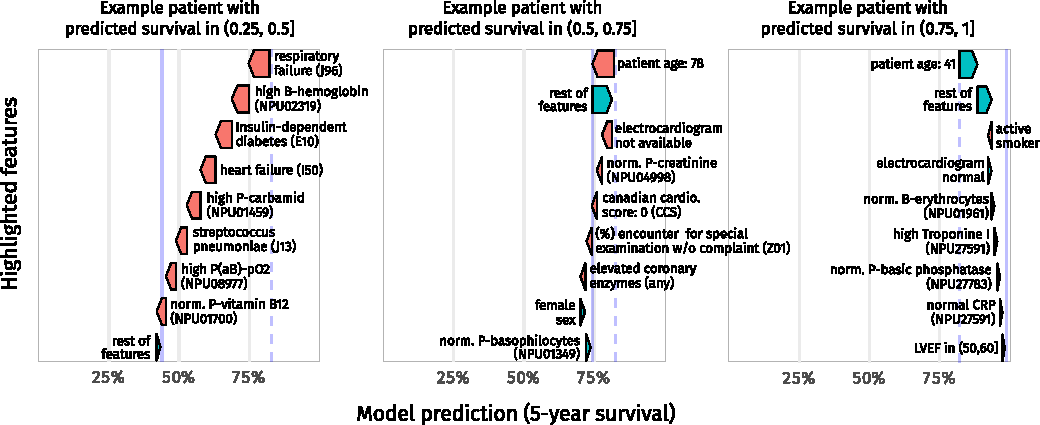
\includegraphics[trim=8mm 5mm 4mm 0]{graphics/pmhnet-v1-shap-individual.pdf}
    \caption[Example patient-level \acs{SHAP} explanations][-2em]{%
        Local patient-level \acsu{SHAP} explanations of 
        5-year predictions from \pmhnet{1}. The three panels shows
        an explanation of the \pmhnet{1} prediction for test-set patients
        with different predicted probability of survival, where 
        each arrow shows the \ac{SHAP} estimated impact of the labeled
        feature on the specific prediction.
        The included patient data have manually been adjusted as to 
        make it non person-sensitive. 
        The vertical dashed lines is the median prediction, and 
        the solid line is the prediction for each patient, which 
        one can obtain by adding all \ac{SHAP} values to the 
        median prediction.}
    \label{fig:shap-individual}
\end{figure}% ←

% figure: shap-overview→
\begin{marginfigure}[-5em]
    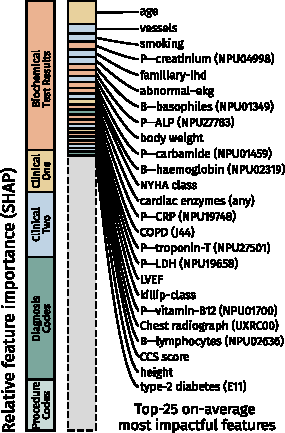
\includegraphics[trim=0 0 0 0]{graphics/pmhnet-v1-feature-impact.pdf}
    \caption[Overview of average feature impact]{%
        By summarising the magnitude of \acsu{SHAP} values, we obtained
        an overview of the relative impact of the different \pmhnet{1} features,
        either aggregated across feature categories (left) or 
        across each individual features (right). 
    }
    \label{fig:shap-overview}
\end{marginfigure}% ←

% figure: shap-dependece-age→
\begin{marginfigure}
    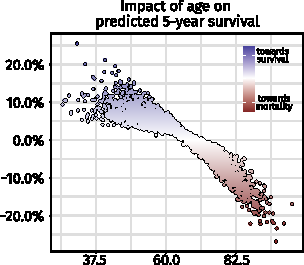
\includegraphics{graphics/pmhnet-v1-shap-age.pdf}
    \caption[\acs{SHAP}-dependence plot for patient age]{%
        Example of a \acs{SHAP} dependence plot 
        showing the \ac{SHAP} value of each \enquote{age} feature
        across the entire test set.}
    \label{fig:shap-dependence-age}
\end{marginfigure}% ←

\section{Conclusion}

In this study, we presented the development and validation of a 
neural network-based discrete time-to-event model for prediction of 
all-cause mortality in patients with \ac{IHD}. 
Our \ac{ML} model, \pmhnet{1}, was found to be well-calibrated and 
to have excellent model discrimination, also in a external cohort 
of \ac{IHD} patients from another country.
Compared to the well-established \graceii{} risk-prediction algorithm,
\pmhnet{1} was found to be significantly better at prediction of all-cause 
mortality.
Furthermore, we showed that by including and utilising a broad array 
of input features, we obtain risk-prediction models with better performance
compared to models only considering a single feature modality and
those limited to a selection of only well-known risk factors.

% Current clinical practice, 
% could potentially benefit from our presented model 
% as it offers better prognostication accuracy than 
% existing alternatives. 
The precise identification of patients at either end of the risk-spectrum,
might be used to select 
patients likely to benefit from more extensive clinical management 
aswell as patients for whom less treatment perhaps 
would be the better option.
However, prospective studies are needed to determine its  impact and
clinical utility.  
Although not part of the included manuscript, 
I have been working together with the public company \acsfont{CIMT}
in the implementation of \pmhnet{1} in \enquote{Sundhedsplatformen}, 
the \ac{EHR} system used in the Capital Region and Region Zealand hospitals.
We succeeded in implementing the model, and there is currently 
an ongoing \ac{RCT} such that the model can be clinically tested.
~\autocite{bundgaardClinical2023}
